\documentclass[conference]{IEEEtran}
\IEEEoverridecommandlockouts
\usepackage{cite}
\usepackage{amsmath,amssymb,amsfonts}
\usepackage{algorithmic}
\usepackage{graphicx}
\usepackage{textcomp}
\usepackage{xcolor}
\usepackage{hyperref}
\usepackage{placeins}
\usepackage[spanish, mexico]{babel}
\def\BibTeX{{\rm B\kern-.05em{\sc i\kern-.025em b}\kern-.08em
    T\kern-.1667em\lower.7ex\hbox{E}\kern-.125emX}}
\usepackage[table,xcdraw]{xcolor}

\title{Modelos de Clasificación con Reseñas de IMDB}

\author{\IEEEauthorblockN{
Dora Alicia Guevara Villalpando \\
Matrícula: 1551003}
\\
\IEEEauthorblockA{\textit{Universidad Autónoma de Nuevo León)} \\
\textit{Facultad de Ciencias Físico Matemáticas}\\
Maestría en Ciencia de Datos \\
Procesamiento y Clasificación de Datos\\\\
dora.guevaravll@uanl.edu.mx}
}

\date{\today}

\begin{document}

\maketitle


\begin{abstract}
Este estudio presenta una comparación de diferentes modelos de clasificación para el análisis de sentimiento en reseñas de películas, se emplea el conjunto de datos IMDB Movie Reviews. Se aplicó un preprocesamiento exhaustivo, seguido de una vectorización con TF-IDF y la evaluación de cuatro modelos de aprendizaje supervisado: Regresión Logística, Support Vector Machines (SVM), Random Forest y Redes Neuronales. Los resultados muestran que la Regresión Logística obtuvo el mejor desempeño con una exactitud del 88.73\%.
\end{abstract}



\section{Introducción}

El análisis de sentimiento es una tarea fundamental en el campo de la minería de texto y el aprendizaje automático. Este tipo de análisis permite identificar las emociones o actitudes expresadas en textos, como positivas, negativas o neutrales. En el contexto de las reseñas de usuarios, es especialmente útil para comprender la percepción del público hacia productos, servicios o contenidos.

En este proyecto, se empleó el conjunto de datos \textit{IMDB Movie Reviews}, que contiene 50,000 reseñas de películas etiquetadas como positivas o negativas. Este dataset es ampliamente utilizado en la comunidad de aprendizaje automático debido a su balance entre clases y la complejidad del lenguaje natural empleado en las reseñas.

El objetivo principal fue desarrollar un modelo capaz de predecir el sentimiento de las reseñas con un alto grado de precisión. Para lograr esto, se exploraron técnicas clásicas de representación de texto y clasificación, evaluando tres enfoques: \textit{Logistic Regression}, \textit{Support Vector Machines (SVM)} y \textit{Random Forest}. Este trabajo también buscó comparar el rendimiento de los modelos para recomendar el más adecuado según las características del dataset y las necesidades del análisis.




\section{Descripción del Conjunto de Datos}

El conjunto de datos utilizado en este estudio es el \textbf{Large Movie Review Dataset v1.0}, desarrollado por Andrew L. Maas et al. (2011) y publicado en la conferencia \textbf{ACL-HLT 2011}. Este dataset es ampliamente utilizado como referencia en tareas de clasificación de sentimientos y contiene reseñas de películas etiquetadas con polaridad positiva o negativa.

\subsubsection{Características del dataset}

\begin{itemize}

	\item Contiene 50,000 reseñas etiquetadas de manera balanceada en 25,000 positivas y 25,000 negativas. Se divide en:
		\begin{itemize}
		\item 25,000 reseñas de entrenamiento (12,500 positivas y 12,500 negativas).
		\item 25,000 reseñas de prueba (12,500 positivas y 12,500 negativas).
		\end{itemize}
	
	\item Cada reseña proviene de una película diferente para evitar sesgos de correlación.
	
\end{itemize}

El dataset está estructurado en carpetas train/ y test/, con subdirectorios pos/ y neg/ que contienen los archivos de texto con las reseñas y sus respectivas etiquetas.

Sin embargo, a pesar que el conjunto de datos originalmente viene separado en \textit{train} y \textit{test} no se considera esto para realizar los análisis presentados a continuación; se opta por juntar ambos conjuntos y trabajar con una base completa con las 50,000 reseñas.



\section{Metodología}

\subsection{Preprocesamiento}

El preprocesamiento de los datos incluyó:

\begin{enumerate}
    \item Limpieza del texto: Se eliminaron etiquetas HTML, caracteres no alfanuméricos y espacios extra.
    
    \item Normalización: Las reseñas se convirtieron a minúsculas para garantizar consistencia.
    
    \item Eliminación de \textit{stop words}: Durante la vectorización, se excluyeron palabras comunes que no aportan información significativa al análisis (como \textit{the}, \textit{and}, entre otras).
\end{enumerate}


\subsection{Conjunto de datos}

El conjunto de datos utilizado, IMDB Movie Reviews, contiene 50,000 reseñas divididas equitativamente en clases positivas y negativas. A pesar de que el dataset original separa los datos en entrenamiento y prueba, en este estudio se optó por combinarlos y realizar una nueva división en un 80\% para entrenamiento y 20\% para prueba.


\subsection{Vectorización}

Para transformar las reseñas en un formato numérico adecuado para los modelos de clasificación, se utilizó el método \textbf{TF-IDF (Term Frequency-Inverse Document Frequency)}. Esta técnica mide la importancia de una palabra dentro de un documento en relación con el corpus completo. Se seleccionó un máximo de 5000 características, lo que permitió capturar las palabras más relevantes sin sobrecargar el modelo con dimensionalidad excesiva.


\subsection{Modelos Evaluados}

\begin{itemize}
    \item \textbf{Logistic Regression:} Este modelo lineal es eficiente y altamente interpretable. Es adecuado para tareas donde las características tienen una relación lineal con las etiquetas de salida.
    
    \item \textbf{Support Vector Machines (SVM):} Utilizando un kernel lineal, este modelo busca maximizar los márgenes entre clases en espacios de alta dimensión, como los generados por TF-IDF.
    
    \item \textbf{Random Forest:} Este enfoque basado en conjuntos utiliza múltiples árboles de decisión para capturar patrones no lineales y manejar datos complejos.

	\item \textbf{Redes Neuronales:} Modelo basado en capas densamente conectadas.    
    
\end{itemize}

Cada modelo fue entrenado utilizando el conjunto de datos de entrenamiento y evaluado en el conjunto de validación. Las métricas clave, como precisión, recall, F1-score y exactitud, fueron utilizadas para comparar su desempeño.



\section{Resultados}

\subsection*{Logistic Regression}

\begin{itemize}
\item \textbf{Precisión}: 0.89 (clase negativa), 0.88 (clase positiva).
\item \textbf{Recall}: 0.88 (clase negativa), 0.90 (clase positiva).
\item \textbf{F1-Score}: 0.88 - 0.89.
\item \textbf{Exactitud Global}: 0.88.
\end{itemize}

\begin{figure}[h]
    \centering
    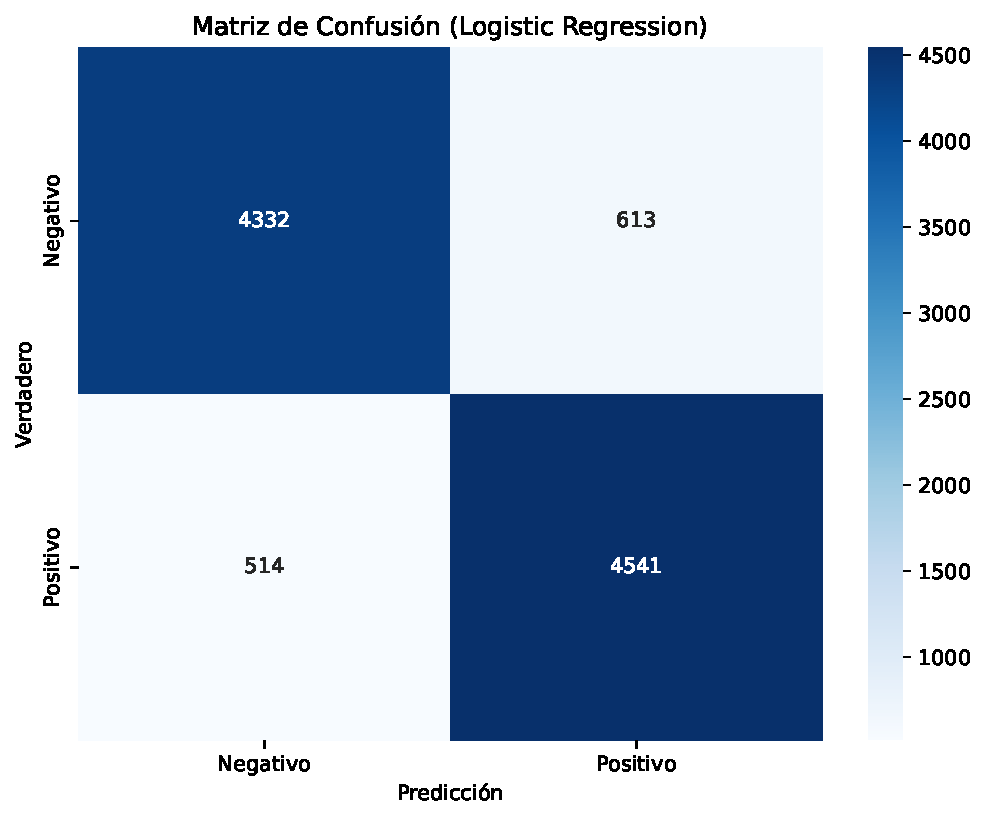
\includegraphics[width=.45\textwidth]{imagenes/matriz_confusion_log_reg.pdf}
    \caption{Matriz de confusion \textit{logistic regression}.}
    \label{fig:log_reg}
\end{figure}

\FloatBarrier


\subsection*{Support Vector Machines (SVM)}

\begin{itemize}
\item \textbf{Precisión}: 0.89 (clase negativa), 0.88 (clase positiva).
\item \textbf{Recall}: 0.88 (clase negativa), 0.89 (clase positiva).
\item \textbf{F1-Score}: 0.88 - 0.89.
\item \textbf{Exactitud Global}: 0.88.
\end{itemize}

\begin{figure}[h]
    \centering
    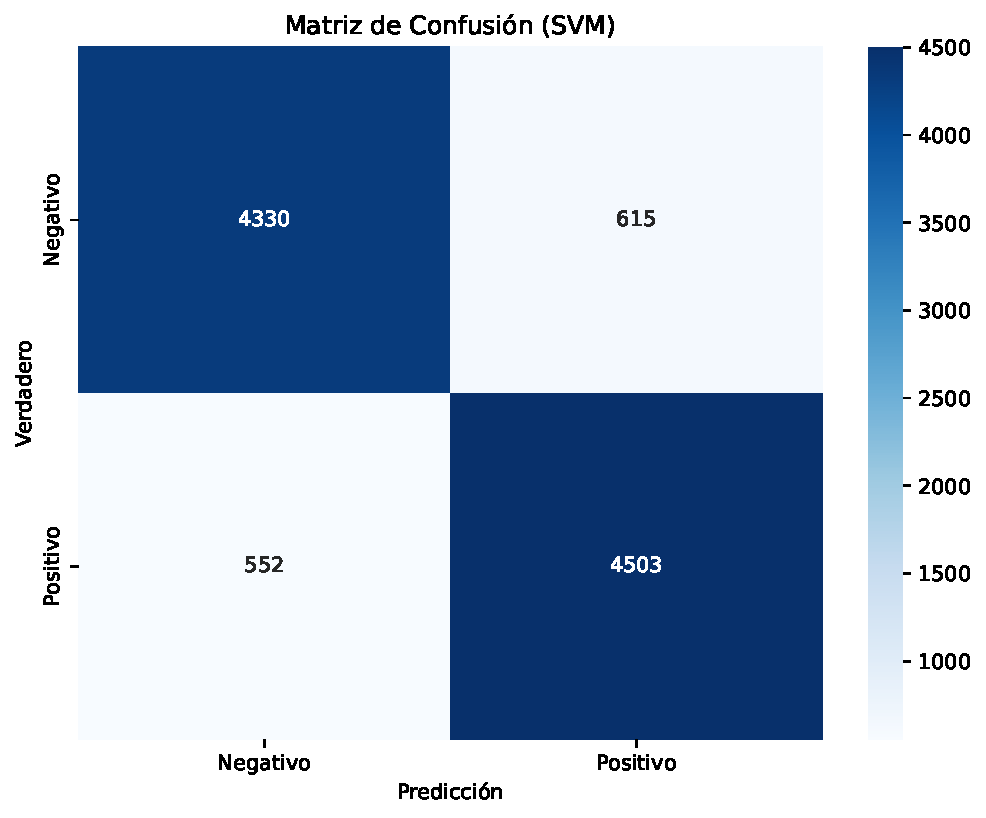
\includegraphics[width=.45\textwidth]{imagenes/matriz_confusion_svm.pdf}
    \caption{Matriz de confusion \textit{SVM}.}
    \label{fig:svm}
\end{figure}

\FloatBarrier


\subsection*{Random Forest}

\begin{itemize}
\item \textbf{Precisión}: 0.83 (clase negativa), 0.85 (clase positiva).
\item \textbf{Recall}: 0.85 (clase negativa), 0.83 (clase positiva).
\item \textbf{F1-Score}: 0.84.
\item \textbf{Exactitud Global}: 0.84.
\end{itemize}

\begin{figure}[h]
    \centering
    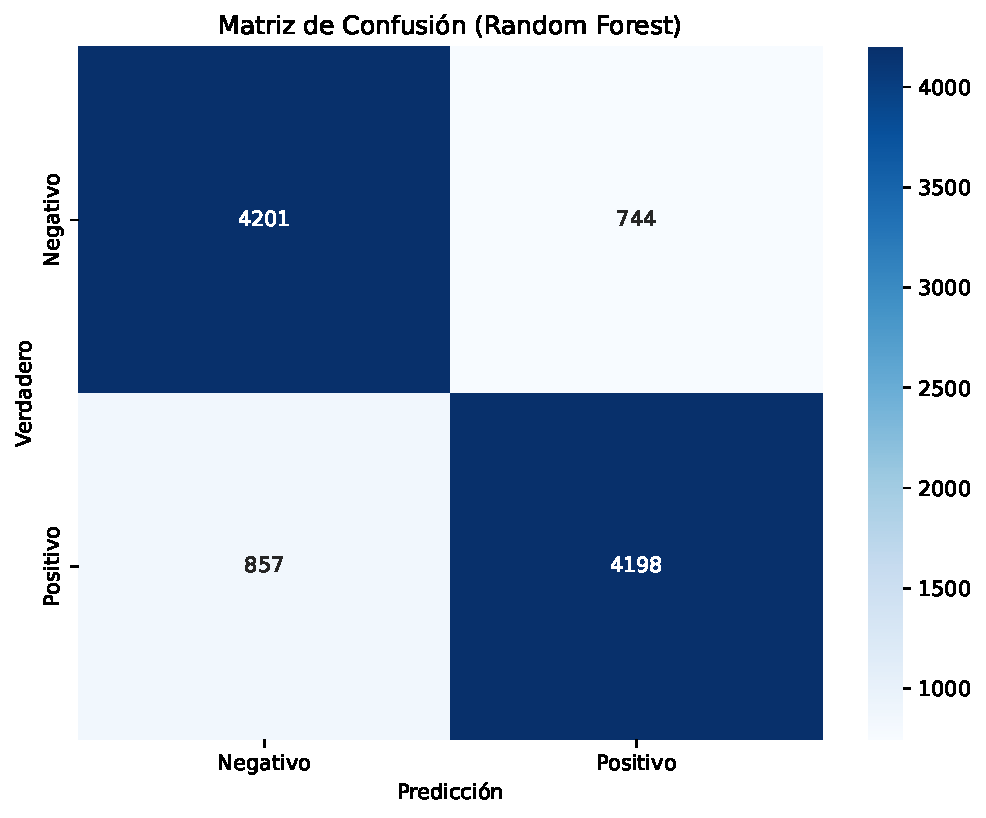
\includegraphics[width=.45\textwidth]{imagenes/matriz_confusion_ran_for.pdf}
    \caption{Matriz de confusion \textit{Random Forest}.}
    \label{fig:rand_f}
\end{figure}

\FloatBarrier

\newpage 

\subsection*{Red Neuronal}

\begin{itemize}
\item \textbf{Precisión}: 0.86 (clase negativa), 0.87 (clase positiva).
\item \textbf{Recall}: 0.87 (clase negativa), 0.86 (clase positiva).
\item \textbf{F1-Score}: 0.86.
\item \textbf{Exactitud Global}: 0.86.
\end{itemize}

\begin{figure}[h]
    \centering
    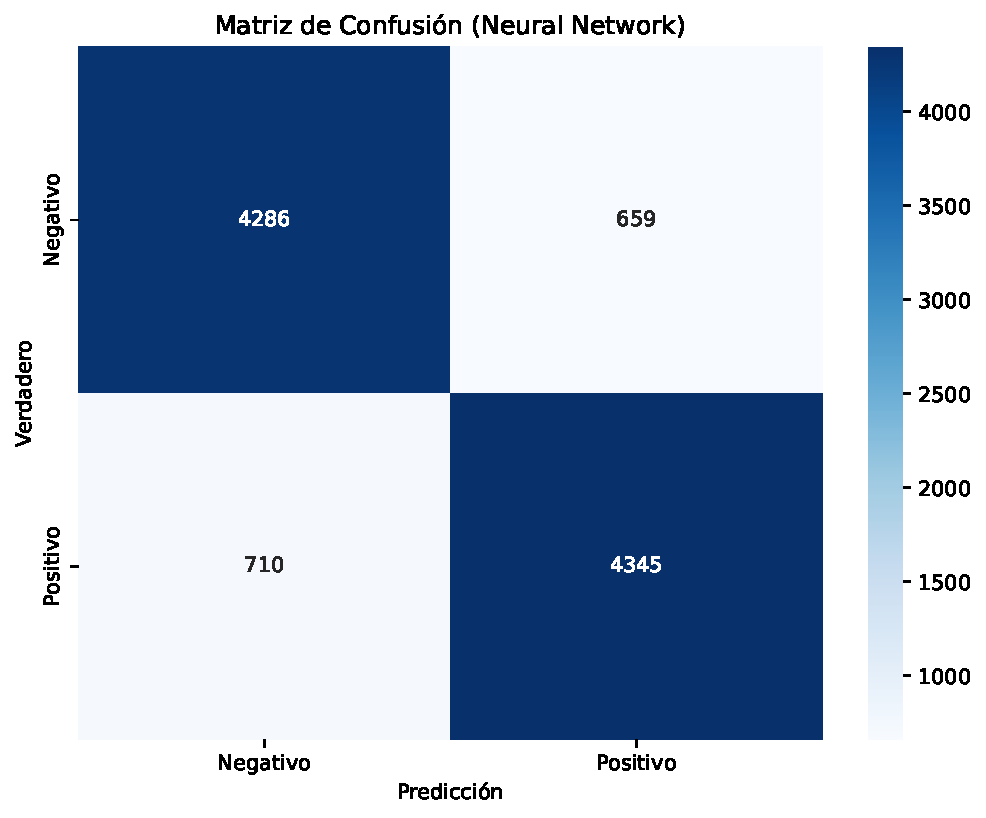
\includegraphics[width=.45\textwidth]{imagenes/matriz_confusion_neural.pdf}
    \caption{Matriz de confusion \textit{Neural Network}.}
    \label{fig:neural}
\end{figure}

\FloatBarrier



\section{Análisis comparativo}

Acorde a lo que se observa en la tabla \ref{tab:comparacion} se puede concluir lo siguiente:
\begin{itemize}
\item Se observa que la Regresión Logística obtuvo el mejor desempeño en términos de exactitud, seguido de SVM y Redes Neuronales. El modelo Random Forest tuvo el peor desempeño en esta tarea.
\end{itemize}


\begin{table}[h!]
    \centering
    \begin{tabular}{ | l | c | c | }
    \rowcolor[HTML]{FFCCC9} 
    \hline
        \multicolumn{1}{c}{\cellcolor[HTML]{FFCCC9}\textbf{Modelo}} & \textbf{Exactitud} & \textbf{F1 Score Promedio} \\ \hline
        Logistic Regression & 88\% & 0.88 \\ \hline
        SVM & 88\% & 0.88 \\ \hline
        Random Forest & 84\% & 0.84 \\ \hline
        Neural Network & 86\% & 0.86 \\ \hline
    \end{tabular}
    \caption{Análisis comparativo}
    \label{tab:comparacion}
\end{table}

\FloatBarrier


En la Figura \ref{fig:comparacion} se muestra un gráfico comparativo entre la exactitud de los modelos.

\begin{figure}[h]
    \centering
    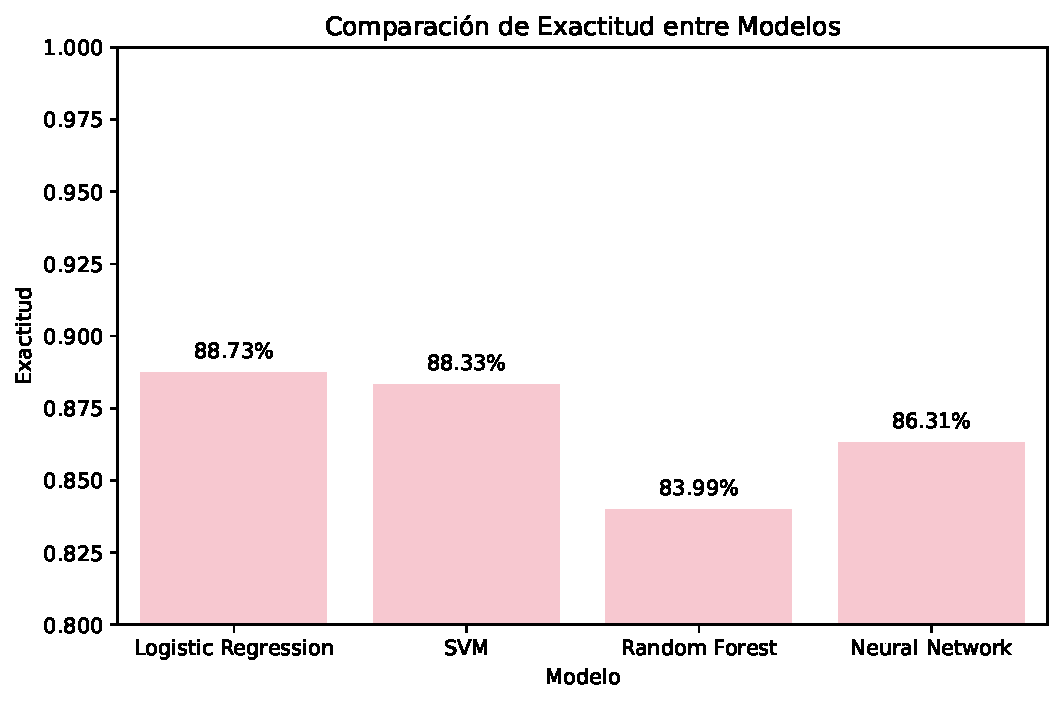
\includegraphics[width=.45\textwidth]{imagenes/Comparacion_Modelos.pdf}
    \caption{Comparación de modelos.}
    \label{fig:comparacion}
\end{figure}

\FloatBarrier


\section{Conclusiones}

Este estudio demostró la efectividad de la Regresión Logística en la clasificación de sentimientos en reseñas de IMDB. Aunque SVM y Redes Neuronales también lograron desempeños competitivos, la simplicidad y eficiencia computacional de la Regresión Logística la hacen una opción viable para aplicaciones en análisis de sentimientos. En trabajos futuros, podría explorarse el uso de modelos de aprendizaje profundo para mejorar los resultados obtenidos.

Tomemos en cuenta los sigueintes puntos:

\begin{enumerate}
    \item \textbf{Modelo Recomendado}:
    \begin{itemize}
        \item \textbf{Logistic Regression} es la mejor opción si se prioriza simplicidad y velocidad.
        \item \textbf{SVM} es una alternativa igualmente válida si se busca robustez en otras configuraciones.
    \end{itemize}
    
    \item \textbf{Modelo Descartado}:
    \begin{itemize}
        \item \textbf{Random Forest}, aunque flexible, no fue competitivo en este escenario.
    \end{itemize}
    
    \item \textbf{Futuras Mejoras}:
    \begin{itemize}
        \item Probar modelos basados en \textit{embeddings} preentrenados como BERT para mejorar el desempeño.
        \item Incrementar el conjunto de datos para explorar el impacto en modelos más complejos.
    \end{itemize}
\end{enumerate}


\section*{Referencias}

\begin{itemize}
    \item Dataset: IMDB Movie Reviews (\url{https://ai.stanford.edu/~amaas/data/sentiment/})

    \item Métodos: Scikit-learn Library (TF-IDF, Logistic Regression, SVM, Random Forest)

    \item Análisis de texto (text mining) con Python. (\url{https://cienciadedatos.net/documentos/py25-text-mining-python}) 
\end{itemize}


\end{document}